% Snowflake Data Engineering — Chapter 14 | original manuscript draft
% Author: Arman Golbidi | Editorial snapshot: 22 October 2026
% Compile: xelatex -interaction=nonstopmode -halt-on-error Snowflake_Data_Engineering_Chapter_13.tex
% Trim: 178 x 254 mm; margins inside 23 mm / outside 17 mm / top-bottom 19 mm.
% Body: 10.75 pt / 13.65 pt leading = 1.27 line-height ratio; code: 8.75 pt.
\documentclass[11pt,twoside]{article}
\usepackage[paperwidth=178mm,paperheight=254mm,inner=23mm,outer=17mm,top=19mm,bottom=19mm,headheight=5mm,headsep=4mm,footskip=9mm]{geometry}
\usepackage{fontspec}
\setmainfont{LibertinusSerif-Regular.otf}[BoldFont=LibertinusSerif-Bold.otf,ItalicFont=LibertinusSerif-Italic.otf,BoldItalicFont=LibertinusSerif-BoldItalic.otf]
\setsansfont{LibertinusSans-Regular.otf}[BoldFont=LibertinusSans-Bold.otf,ItalicFont=LibertinusSans-Italic.otf]
\setmonofont{LibertinusMono-Regular.otf}[Scale=0.91]
\usepackage[english]{babel}
\usepackage{microtype}
\usepackage{setspace}
\setstretch{1.0}
\usepackage{titlesec,enumitem,tabularx,array,booktabs,needspace,fancyhdr,lastpage}
\usepackage[most]{tcolorbox}
\usepackage{tikz}
\usetikzlibrary{arrows.meta,positioning,fit,shapes.misc,calc}
\usepackage{listings}
\usepackage{xcolor}
\usepackage{hyperref}
\usepackage{amsmath}
\hypersetup{colorlinks=true,urlcolor=steelblue,linkcolor=steelblue,pdfauthor={Arman Golbidi},pdftitle={Snowflake Data Engineering - Chapter 14: Snowflake Cortex AI and Machine Learning},pdfsubject={English technical book manuscript, fourteenth chapter, 178 x 254 mm}}
\definecolor{navy}{HTML}{15334A}
\definecolor{steelblue}{HTML}{17779B}
\definecolor{teal}{HTML}{12888A}
\definecolor{lightblue}{HTML}{ECF5F7}
\definecolor{papergray}{HTML}{F2F5F6}
\definecolor{inkgray}{HTML}{4A5862}
\definecolor{thinrule}{HTML}{CBD7DB}
\AtBeginDocument{\color{navy}\fontsize{10.75}{13.65}\selectfont}
\setlength{\parindent}{0pt}
\emergencystretch=2.5em
\setlength{\parskip}{3.3pt plus 0.7pt minus 0.6pt}
\setlist[itemize]{leftmargin=4mm,itemsep=1pt,topsep=2pt,parsep=0pt}
\setlist[enumerate]{leftmargin=5mm,itemsep=1pt,topsep=2pt}
\titleformat{\section}{\sffamily\bfseries\color{navy}\fontsize{14}{17}\selectfont}{}{0pt}{}
\titlespacing*{\section}{0pt}{8pt}{4pt}
\titleformat{\subsection}{\sffamily\bfseries\color{steelblue}\fontsize{10.8}{13}\selectfont}{}{0pt}{}
\titlespacing*{\subsection}{0pt}{5pt}{1pt}
\newcommand{\topic}[2]{\subsection*{#1\quad #2}}
\newcommand{\repo}[2]{\par\begingroup\fontsize{8.0}{9.6}\selectfont\sffamily\color{inkgray}\textbf{Project reference:} \href{#2}{#1}. \textit{Not independently executed; rights review pending.}\par\endgroup}
\newtcolorbox{insight}[1][]{enhanced,breakable,colback=lightblue,colframe=thinrule,boxrule=.45pt,arc=1.3mm,left=2.8mm,right=2.8mm,top=1.8mm,bottom=1.8mm,before skip=5pt,after skip=5pt,#1}
\newtcolorbox{whitebox}[1][]{enhanced,breakable,colback=papergray,colframe=thinrule,boxrule=.35pt,arc=1mm,left=2.6mm,right=2.6mm,top=1.5mm,bottom=1.5mm,before skip=4pt,after skip=5pt,#1}
\lstdefinestyle{chaptercode}{basicstyle=\ttfamily\fontsize{8.75}{10.7}\selectfont,backgroundcolor=\color{papergray},frame=single,framerule=.35pt,rulecolor=\color{thinrule},breaklines=true,columns=fullflexible,keepspaces=true,showstringspaces=false,aboveskip=5pt,belowskip=5pt,xleftmargin=2mm,xrightmargin=1mm,framexleftmargin=2mm,framexrightmargin=1mm}
\lstset{style=chaptercode}
\pagestyle{fancy}
\fancyhf{}
\fancyhead[LE]{\sffamily\fontsize{7.6}{9}\selectfont\color{inkgray}\textsc{Snowflake Data Engineering}}
\fancyhead[RO]{\sffamily\fontsize{7.6}{9}\selectfont\color{inkgray}\textsc{14 / Cortex AI \& ML}}
\fancyfoot[LE,RO]{\sffamily\bfseries\fontsize{8.2}{9}\selectfont\color{steelblue}\thepage}
\fancyfoot[LO,RE]{\sffamily\fontsize{7.6}{9}\selectfont\color{inkgray}Arman Golbidi \quad | \quad Chapter 14}
\renewcommand{\headrulewidth}{0.35pt}
\renewcommand{\footrulewidth}{0pt}
\setcounter{page}{249}
\raggedbottom

\begin{document}
% PAGE 249
{\sffamily\bfseries\fontsize{9}{11}\selectfont\color{steelblue} CHAPTER 14 \hfill EVALUATION / EVIDENCE / COST}\par\vspace{3mm}
{\sffamily\bfseries\fontsize{20}{23}\selectfont\color{navy} Snowflake Cortex AI\\and Machine Learning}\par\vspace{2mm}
{\sffamily\fontsize{11}{14}\selectfont\color{steelblue} Does a model improve the decision, or only make the system more complicated?}\par\vspace{3mm}
\begin{insight}\textbf{An appealing forecast is not yet a useful forecast.}\par
The Finland Energy Analytics dashboard has a carefully validated, synthetic history and a clear metric contract. Someone proposes adding an AI assistant that predicts tomorrow's generation and answers operational questions. A colourful curve appears quickly; the actual task is harder. Could yesterday's value or last week's value predict as well? Was future information leaked into training? Will the assistant invent a data source? Who pays for repeated prompts, and where are those prompts processed?
\end{insight}
Chapter~13 established access controls, provenance, runbooks and workload budgets. Here those controls become prerequisites for model development. Machine learning (ML) estimates patterns from observations; generative AI produces content from learned distributions. Neither automatically makes data accurate or a forecast actionable. The engineer must define a decision, preserve a chronological holdout, measure error, inspect failures and record the cost of each alternative.
\begin{whitebox}\textbf{Learning outcomes}\par
By the end, you should be able to (1) decide whether SQL, statistics, ML or a language model fits a task; (2) evaluate Cortex availability and inference residency; (3) design and test AI SQL prompts; (4) explain grounded retrieval and natural-language analytics; (5) build leakage-safe energy features; (6) compare naive and seasonal forecasting baselines; (7) write a model card; and (8) estimate and monitor AI-related credit usage without assuming a universal price.
\end{whitebox}
\textbf{Prerequisites.} Chapters~9, 11--13, elementary Python, basic notions of forecast error and Snowflake roles. All printed sample observations and scores are explicitly synthetic. The offline lab needs only the Python standard library; optional AI calls require permission, supported models/regions and billing approval.
\begin{center}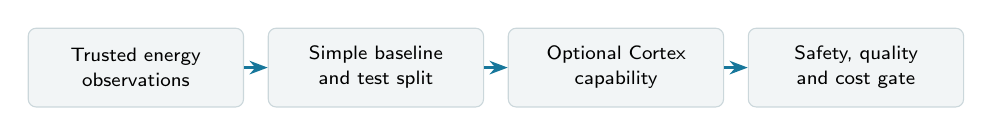
\begin{tikzpicture}[>=Stealth,every node/.style={font=\sffamily\fontsize{7.5}{9}\selectfont},n/.style={draw=thinrule,rounded corners=1mm,fill=papergray,align=center,text width=25mm,minimum height=10mm}]
\node[n](a){Trusted energy\\observations};\node[n,right=3mm of a](b){Simple baseline\\and test split};\node[n,right=3mm of b](c){Optional Cortex\\capability};\node[n,right=3mm of c](d){Safety, quality\\and cost gate};
\draw[->,thick,steelblue](a)--(b);\draw[->,thick,steelblue](b)--(c);\draw[->,thick,steelblue](c)--(d);
\end{tikzpicture}\\{\fontsize{8}{9}\selectfont\color{inkgray}Figure 14.1. Prove a baseline before introducing a billable AI extension.}\end{center}

\newpage

% PAGE 250
\section*{14.1\quad AI/ML use cases in a modern data platform}
\topic{14.1.1}{Choose a workload, not a fashionable model}
An energy engineer can use ordinary SQL to total generation, flag negative readings or join a device dimension. Deterministic rules should remain deterministic: an AI-generated answer to a calculation already defined by a validated SQL expression adds uncertainty with little value. ML is more appropriate when the sought relationship is uncertain: estimating load one day ahead, ranking likely faults or detecting unexpected behaviour in an evolving time series. A language model can help interpret unstructured incident notes, but it cannot replace the measured fact table.

\begin{center}\small\begin{tabularx}{\linewidth}{@{}p{27mm}X X@{}}\toprule
Question & First credible method & Why it fits \\ \midrule
How much energy? & SQL aggregate & Exact, reproducible arithmetic \\
Is reading valid? & Typed rule and contract & Explicit threshold and failure reason \\
What will happen? & Naive / seasonal forecast & Testable prediction benchmark \\
Why was equipment stopped? & Search plus cited notes & Unstructured evidence and provenance \\
Which action to take? & Human-governed decision & Requires operational accountability \\
\bottomrule\end{tabularx}\end{center}
\topic{14.1.2}{Value, failure impact and permitted data}
Express value as a decision with a measurable consequence. A grid scheduling assistant might reduce manual inspection time, but a false ``normal'' designation might delay maintenance. Prioritise use cases by expected value, error severity, required freshness, observability, sensitivity, and whether a human can reject a suggestion. A promising proof of concept may still be unsuitable for unattended operation.

A data contract precedes a model contract. Confirm ownership, licensing, retention and lawful processing for each input: raw telemetry, operator notes and external weather predictions can have different constraints. A prompt is a data transfer, not a harmless string. Minimise sensitive data, retain structured identifiers needed for provenance, and evaluate downstream sharing rules for generated summaries.
\begin{insight}\textbf{Decision checkpoint.} If errors can be described and fixed with an approved SQL condition, choose SQL. If success requires estimating an unknown target from past observations, compare statistical and ML baselines. If the input is narrative text, test retrieval or AI-assisted extraction with an audit trail rather than accepting an unsupported explanation.\end{insight}
\repo{P156: getting started with machine learning}{https://github.com/Snowflake-Labs/sfguide-getting-started-machine-learning}

\newpage

% PAGE 251
\topic{14.1.3}{Build an evaluation baseline before an AI prototype}
A model comparison is meaningful only if every candidate receives the same input rights, prediction time, validation windows and scoring procedure. For daily energy forecasting, choose a forecast horizon (tomorrow), a unit (MWh per day), a decision consumer (planning analyst), and a loss function (for example, mean absolute error, MAE). Specify the acceptable error\emph{ before} seeing model scores. Record the timestamp at which each predictor would actually have been known.

Our running energy case offers six accepted generation observations totalling 66.000 MWh in the earlier chapters. Six observations cannot demonstrate a trustworthy multiweek forecast. Therefore Chapter~14 creates an \emph{additional, explicitly synthetic} 35-day teaching series with a weekly cycle and one artificial spike. These rows are neither sampled Finnish energy measurements nor copied observations; they exist to test chronological splits, naive predictions and anomaly alert logic under controlled conditions.

A minimum experiment has three comparisons: a last-value forecast ($\hat y_t=y_{t-1}$), a seasonal last-week forecast ($\hat y_t=y_{t-7}$), and an optional learned model evaluated on the same held-out days. A language-model-generated narrative is assessed separately for factual consistency and evidence support; its fluency is not a numeric forecasting score.
\begin{whitebox}\textbf{Pre-registered experiment card}\par
\textbf{Input:} synthetic daily generation; one observation per UTC date. \textbf{Split:} days 0--20 train, 21--27 validation, 28--34 final test. \textbf{Prediction horizon:} one day. \textbf{Baselines:} lag 1 and lag 7. \textbf{Metrics:} test MAE plus anomaly false/true positives. \textbf{Guardrail:} future target values may not appear as current features. \textbf{Decision:} add a complex model only if it beats the seasonal baseline and meets safety/cost requirements.
\end{whitebox}
\textbf{Common failure.} Randomly shuffle a chronological series before splitting and train a model on tomorrow's meter reading to predict tomorrow's meter reading. The resulting high accuracy measures leakage, not predictive ability. In production, holdouts should include shifts in season, holidays, missing sensors and regime changes; our tiny lab does not establish reliability in those conditions.

\textbf{Check.} Write a one-sentence claim about improvement that could be \emph{falsified} by a future test, not one that merely describes how sophisticated the model is.

\newpage

% PAGE 252
\section*{14.2\quad Cortex AI capabilities and availability caveats}
\topic{14.2.1}{Separate product families and operational jobs}
The Snowflake AI and ML portfolio spans managed AI SQL functions for text and multimodal inputs; search services supporting retrieval-augmented generation (RAG); semantic natural-language analytics; and ML capabilities for forecasting, anomaly detection and model development. The functions answer different questions. For example, \texttt{AI\_CLASSIFY} assigns supplied categories; \texttt{AI\_COMPLETE} generates responses; a search service retrieves relevant indexed text; a forecasting model estimates a numeric trajectory. Treat ``Cortex'' as a product family, not one uniform endpoint or billing meter.\footnote{Snowflake documentation: \url{https://docs.snowflake.com/en/user-guide/snowflake-cortex/llm-functions} and \url{https://docs.snowflake.com/en/user-guide/snowflake-cortex/cortex-search/cortex-search-overview}.}
\topic{14.2.2}{Availability is account-specific}
Feature status, model allow-lists, access privileges, region, cloud provider, and preview restrictions change. The same SQL identifier can be valid in one account and unavailable in another. Before a paid trial, have an administrator review the documented function privileges, model lifecycle, available models and the account's relevant feature/edition constraints. In 2026, Cortex model RBAC and allow-lists have become important enforcement points; never infer permission from the ability to query a conventional table.
\begin{lstlisting}[language=SQL]
-- Read-only account check; admin may need to perform it.
SHOW PARAMETERS LIKE 'CORTEX_ENABLED_CROSS_REGION'
  IN ACCOUNT;
-- Additional model/feature listings vary by privilege.
\end{lstlisting}
\topic{14.2.3}{Storage residency is not inference residency}
Data stored in an account region can still be sent temporarily to a permitted processing region if cross-region inference is enabled. The request payload and generated answer may cross a regional boundary. A strict data-residency policy therefore requires a specific review of inference routing, not only the location of source tables. Do not change the account-level \texttt{CORTEX\_ENABLED\_CROSS\_REGION} parameter from a teaching notebook; it is an administrator-controlled governance decision.
\begin{insight}\textbf{Deployment gate.} Record home cloud/region; supported processing region; model ID and lifecycle; approved inference route; sensitive input classification; relevant privilege; anticipated usage; and owner approval. ``Available somewhere'' is not evidence of local availability or compliance.\end{insight}
\repo{P157: Cortex AI functions guide}{https://github.com/Snowflake-Labs/sfguide-getting-started-with-cortex-ai-functions}

\newpage

% PAGE 253
\section*{14.3\quad AI SQL functions and evaluation principles}
\topic{14.3.1}{Understand AI SQL semantics before writing queries}
A conventional SQL aggregate is deterministic given unchanged data and query semantics. An AI function evaluates an input using a managed model and may be probabilistic, evolve over time or return an error/NULL for a subset of rows. Do not equate the presence of a result with correctness. Snowflake documents \texttt{AI\_COMPLETE}, \texttt{AI\_CLASSIFY}, \texttt{AI\_SUMMARIZE} and other functions; exact function signatures, available models, error behaviour and privileges require a documentation check before deployment.

\begin{lstlisting}[language=SQL]
-- OPTIONAL BILLABLE EXAMPLE. Test in an approved sandbox.
-- The model identifier must be checked for your account.
SELECT AI_CLASSIFY(
  'Turbine B was offline after an inverter alarm',
  ['maintenance', 'operations', 'commercial']
) AS suggested_category;
\end{lstlisting}
The classification should be compared with a human-labeled answer. Even a syntactically valid label might be unsupported by the note. For a multi-label task, decide whether several classes are acceptable; for an exclusive taxonomy, define what to do when the model gives more than one or no recognized category.
\topic{14.3.2}{Prompts are interfaces with contracts}
A reliable prompt identifies the task, permitted context, output type, evidence rules, fallback and forbidden behaviour. Consider an incident-summary assistant: it must distinguish a confirmed diagnosis from a technician's hypothesis, preserve the original device identifier, not invent measured outage duration, and answer ``insufficient evidence'' when the note is ambiguous. Put required output fields in a validated schema and enforce application-side type checks after inference.
\begin{whitebox}\textbf{Proposed output contract}\par
\texttt{incident\_id}: identifier from source; \texttt{summary}: short statement grounded in the note; \texttt{category}: one of the approved labels; \texttt{evidence\_spans}: quoted source spans/offsets; \texttt{needs\_review}: boolean. Reject unknown keys or references to nonexistent source spans. This contract is original example logic, not a claim that every model will follow it unaided.
\end{whitebox}
\textbf{Failure path.} If the model returns malformed JSON or a confident diagnosis absent from the note, quarantine the response and retain the input hash, model ID, version/time and evaluation status. Never silently coerce unrecognized categories into ``normal''.

\newpage

% PAGE 254
\topic{14.3.3}{Build labelled cases and measure more than fluency}
An evaluation set should include typical, rare, adversarial and intentionally unanswerable inputs. For the energy incident assistant, include a clear inverter alarm, a contradictory maintenance note, a prompt-injection sentence embedded in a source note, an incident with no device ID, a multilingual note and an explicit ``no known cause'' example. Source text is evidence to be interpreted, not instructions to override the assistant's task.

\begin{center}\small\begin{tabularx}{\linewidth}{@{}p{26mm}p{28mm}X@{}}\toprule
Dimension & Metric & A practical failure test \\ \midrule
Classification & Precision, recall, F1 & Confusing cause with symptom \\
Extraction & Field accuracy & Invented device identifier \\
Grounding & Citation support rate & Citation does not contain claim \\
Abstention & Correct refusal rate & Answer despite absent evidence \\
Safety & Rule-violation count & Source note attempts prompt override \\
Operation & Latency and credits & Large prompt repeated across many rows \\
\bottomrule\end{tabularx}\end{center}
In a classification experiment, report a confusion matrix and the number of examples, not a single vague ``accuracy'' statement. Human raters need a consistent rubric; disagreements should be adjudicated, and labels must be stored independently of model outputs. Evaluate at least once on a frozen holdout set not used to refine prompts.

\textbf{The workflow matters as much as the score.} Fix prompt template and model before a batch evaluation. Capture failures as evidence, revise in a separate development cycle, and rerun the unchanged final holdout. A retrieval component can be evaluated independently (did it find the correct note?) before the generation component (did it use only retrieved evidence?). This helps distinguish missing information from invented content.
\begin{insight}\textbf{Metric integrity.} Suppose 18 of 20 incident summaries cite the right document, but only 12 cite a span supporting their central claim. ``90\% contain a citation'' is not evidence that 90\% are grounded. Prefer a claim-level evidence check and include the denominator and confidence limitations.
\end{insight}
\repo{P161: prompt engineering and LLM evaluation}{https://github.com/Snowflake-Labs/sfguide-prompt-engineering-and-llm-evaluation}
\textbf{Check.} Which metric should trigger an immediate human-review requirement, even if a model's overall score improves?

\newpage

% PAGE 255
\section*{14.4\quad Search, retrieval, and natural-language analytics}
\topic{14.4.1}{Retrieve evidence before composing a response}
Retrieval-augmented generation (RAG) brings permitted supporting records to the model at question time. A search service indexes selected content and returns candidate passages. A generation step then answers with explicit citations to those passages. Cortex Search uses a mixture of lexical and semantic matching with reranking; quality still depends on source coverage, freshness, permission design, chunking and relevance. Unlike a static glossary, an index can incur refresh, embedding and serving charges.
\begin{center}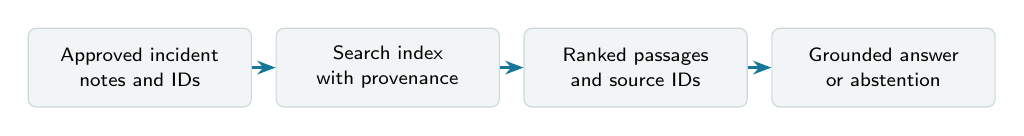
\begin{tikzpicture}[>=Stealth,every node/.style={font=\sffamily\fontsize{7.5}{9}\selectfont},n/.style={draw=thinrule,rounded corners=1mm,fill=papergray,align=center,text width=26mm,minimum height=10mm}]
\node[n](a){Approved incident\\notes and IDs};\node[n,right=3mm of a](b){Search index\\with provenance};\node[n,right=3mm of b](c){Ranked passages\\and source IDs};\node[n,right=3mm of c](d){Grounded answer\\or abstention};
\draw[->,thick,steelblue](a)--(b);\draw[->,thick,steelblue](b)--(c);\draw[->,thick,steelblue](c)--(d);
\end{tikzpicture}\\{\fontsize{8}{9}\selectfont\color{inkgray}Figure 14.2. Retrieval narrows evidence; it does not prove that generated claims are true.}\end{center}
\topic{14.4.2}{Attribution and the hidden access boundary}
A useful answer records source document ID, excerpt, version and retrieval timestamp, with claim-level citation checks. If an incident report is reclassified as restricted, refresh paths and cached/indexed copies also require review. Search-service access can operate with owner-rights semantics; a user permitted to query a service may see indexed rows unless the service is designed with appropriate per-user boundaries. Do not assume a row-access policy on a source table is automatically applied during every search response.\footnote{See the official Cortex Search overview and its access-control discussion: \url{https://docs.snowflake.com/en/user-guide/snowflake-cortex/cortex-search/cortex-search-overview}.}
\topic{14.4.3}{Natural-language SQL needs semantic constraints}
Cortex Analyst turns business questions into SQL-oriented responses using a defined semantic interpretation of tables and metrics. ``Energy generated'' must carry the right unit, grain, filters and sign conventions; otherwise a plausible query can be numerically wrong. Apply an allow-list of approved serving views, inspect generated SQL where applicable, restrict execution privileges and verify result totals against certified KPI queries. The system is not a substitute for a trusted metric contract.
\repo{P162: document RAG with Cortex Search}{https://github.com/Snowflake-Labs/sfguide-ask-questions-to-your-documents-using-rag-with-snowflake-cortex-search}

\newpage

% PAGE 256
\section*{14.5\quad Data preparation and feature engineering with Snowpark}
\topic{14.5.1}{A time series is not merely a sorted CSV}
Time-based predictions depend on a canonical business grain. The energy fact from previous chapters is keyed by source, metric and event time, while today's forecasting lab uses one aggregate generation value for each UTC date. First determine whether missing days mean zero generation, missing telemetry or a source outage. Never fill a missing day with zero without a domain rule: this creates artificial collapses that may look like anomalies.

In Snowpark, use warehouse-side filters and aggregations rather than collecting unrestricted raw data to a laptop. A preparation query might collapse approved hourly readings into UTC days, check valid units, remove superseded revisions and retain an \texttt{as\_of} timestamp for reproducibility. Only after that contract is satisfied should Python create forecasting features.
\begin{lstlisting}[language=SQL]
-- Illustration: use an approved, unique daily-serving view.
SELECT DATE_TRUNC('DAY', event_time_utc)::DATE AS d,
       SUM(generation_mwh) AS total_mwh
FROM BOOK_CH14.GOLD.V_ENERGY_ACCEPTED
WHERE event_time_utc < :as_of_utc
GROUP BY 1 ORDER BY 1;
-- View and bind variable are illustrative prerequisites.
\end{lstlisting}
\topic{14.5.2}{Construct past-only lag and rolling features}
The lag-7 feature for day $t$ is $y_{t-7}$. A seven-day rolling average predicting day $t$ should use $y_{t-1},\ldots,y_{t-7}$, \emph{not} $y_t$. The difference is one misplaced window boundary. For a one-day-ahead forecast made at the end of day $t-1$, weather forecasts issued before that time may be eligible predictors; realized temperatures for day $t$ are not.
\begin{lstlisting}[language=SQL]
-- Conceptual Snowflake window; verify grain and order.
SELECT d, total_mwh,
       LAG(total_mwh, 7) OVER (ORDER BY d) AS lag_7,
       AVG(total_mwh) OVER (
         ORDER BY d ROWS BETWEEN 7 PRECEDING
                            AND 1 PRECEDING) AS avg_7_past
FROM BOOK_CH14.GOLD.V_DAILY_ENERGY;
\end{lstlisting}
A row-number window assumes one row per calendar day; otherwise a lag of seven rows is not seven days. Validate continuity before applying it. Keep the feature transformation and any imputation policy in version-controlled code so evaluation and serving use identical logic.

\newpage

% PAGE 257
\topic{14.5.3}{Split by time and freeze the training view}
For the synthetic 35-day lab, day indices 0--20 supply training history, 21--27 are a validation interval and 28--34 form a sealed test interval. Set hyperparameters on training/validation data, and compute the final score only once for the chosen design. The seasonal baseline does not ``fit'' coefficients, but its anomaly threshold is calibrated from validation residuals, not from the test spike.

A deployment often requires a \emph{rolling-origin} evaluation rather than one lucky holdout: train to an early cutoff, predict the next horizon, advance the cutoff and repeat. When a source has multiple devices, group identifiers and time boundaries carefully; mixing measurements from the same physical incident across train and test can leak its signature. Compare forecasts at the exact lead time required by the operational decision.
\begin{center}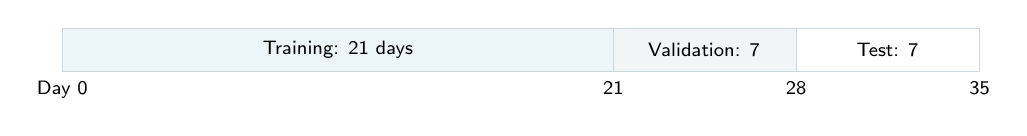
\begin{tikzpicture}[every node/.style={font=\sffamily\fontsize{7.3}{9}\selectfont}]
\draw[fill=lightblue,draw=thinrule] (0,0) rectangle (7.0,.55);
\draw[fill=papergray,draw=thinrule] (7,0) rectangle (9.32,.55);
\draw[fill=white,draw=thinrule] (9.32,0) rectangle (11.65,.55);
\node at (3.5,.28){Training: 21 days};\node at (8.15,.28){Validation: 7};\node at (10.48,.28){Test: 7};
\node[below] at (0,0){Day 0};\node[below] at (7,0){21};\node[below] at (9.32,0){28};\node[below] at (11.65,0){35};
\end{tikzpicture}\\{\fontsize{8}{9}\selectfont\color{inkgray}Figure 14.3. Chronological evaluation prevents test outcomes from choosing the model.}\end{center}
\begin{whitebox}\textbf{Leakage checklist}\par
(1) Is every training record timestamped before the cutoff? (2) Were late revisions frozen as they were known at inference time? (3) Are window features shifted correctly? (4) Is the scaling or imputation fitted only on past values? (5) Were thresholds fixed without looking at test errors? (6) Can the exact feature table be reconstructed from its inputs and \texttt{as\_of} metadata?
\end{whitebox}
\textbf{Trade-off.} Snowpark and an in-platform feature store can centralise governance, but introduce additional objects and operational costs; a modest, fixed SQL view may be sufficient for a small forecasting application. Select infrastructure only after identifying reuse, update frequency and access boundaries.
\repo{P165: ML feature engineering in Python}{https://github.com/Snowflake-Labs/sfguide-intro-to-machine-learning-with-snowflake-ml-for-python}

\newpage

% PAGE 258
\section*{14.6\quad Forecasting and anomaly detection use cases}
\topic{14.6.1}{Naive baselines make sophisticated claims falsifiable}
The last-value prediction assumes tomorrow resembles today: $\hat y_t=y_{t-1}$. The seasonal naive baseline repeats the same weekday one week ago: $\hat y_t=y_{t-7}$. Both are cheap, interpretable and defensible first benchmarks. If an ML model cannot consistently improve on these at the required lead time, its maintenance and inference bill require special justification.
\topic{14.6.2}{Forecasts, alarms and operational thresholds are different}
A forecast answers ``how much?'' An anomaly detector answers ``is this observation unexpectedly different from a justified reference?'' A maintenance decision asks ``what should someone do?'' Those are three distinct stages. Our offline lab uses \emph{seasonal residuals} $e_t=|y_t-y_{t-7}|$ and sets a threshold from the earlier validation period, then injects an artificial spike on the final test day. This is a teaching heuristic, \emph{not} an industry-calibrated prediction interval or production fault detector.
\begin{lstlisting}[language=Python]
# Excerpt from accompanying ml_baseline.py
seasonal = values[t - 7]  # known at prediction time
error = abs(values[t] - seasonal)  # scoring afterwards
alert = error > threshold  # threshold fixed from validation
\end{lstlisting}
Snowflake ML also documents managed forecasting and anomaly-detection objects in the \texttt{SNOWFLAKE.ML} namespace. Those are optional comparative systems, not hidden prerequisites for the offline script. In a live experiment, first verify input-shape constraints and training history requirements; preserve result history and the model's own evaluation metadata.
\topic{14.6.3}{Score both error and confidence honestly}
Mean absolute error is $\mathrm{MAE}=n^{-1}\sum_t |y_t-\hat y_t|$ in MWh, directly interpretable at the original unit. Percentage errors become unstable near zero generation; use care with MAPE and report the count of zero targets. An interval's usefulness requires empirical coverage on unseen data, not merely a visually wide shaded region. For alarms, track missed events, false alerts, time-to-detection and whether humans actually changed an action.
\begin{insight}\textbf{Verified offline fixture (not a Snowflake benchmark).} On seven held-out synthetic days the seasonal baseline scores \textbf{1.0643 MWh MAE}; last-value scores \textbf{3.2500 MWh MAE}. A validation-derived threshold flags the one injected test spike (index 34). With one deliberately placed event, this does not estimate a real-world detection rate.\end{insight}
\repo{P010: predictive grid maintenance case study}{https://github.com/Snowflake-Labs/sfguide-ai-powered-predictive-grid-maintenance}

\newpage

% PAGE 259
\section*{14.7\quad Model evaluation, security, and responsible AI}
\topic{14.7.1}{Model permissions and data permissions form one boundary}
A secured warehouse view is not sufficient if an application forwards its raw fields into a broader model invocation. Authorisation must cover the service principal, eligible input columns, region processing route, model family, produced artefacts, logs, and users allowed to read those outputs. Deny sensitive incident notes by default; introduce a reviewed, minimised view for a specific approved use case.

For Cortex AI Functions, access involves the appropriate Snowflake database role and, depending on the model, model-specific access control and account allow-lists. In contrast, an externally hosted application may add network policies, secret rotation and vendor contracts. A model registry does not automatically authorise serving. Use a narrow execution role for training and a separate role for inference and publication.
\topic{14.7.2}{Reproducibility includes human judgment}
Retain the dataset fingerprint, split dates, code commit, feature version, model name, settings, scoring script, error examples and reviewer decision. Avoid placing raw sensitive prompts in indiscriminate diagnostics. For a human-in-the-loop workflow, show the source evidence next to the model suggestion and allow reviewers to reject it, flag an unsupported claim, or correct an incident category. Their overrides become auditable labels rather than invisible manual fixes.
\begin{whitebox}\textbf{Promotion evidence packet}\par
\textbf{Purpose:} energy planning assistance. \textbf{Data:} approved synthetic prototype, then governed operational slice. \textbf{Validation:} chronological, named holdouts. \textbf{Baseline:} seasonal naive. \textbf{Model:} exact identifier, lifecycle and settings. \textbf{Safety:} access denial and evidence attribution cases. \textbf{Operator:} named owner, rollback procedure. \textbf{Cost:} measured credits or declared assumptions. \textbf{Approval:} signed decision with unresolved limitations.
\end{whitebox}
If a model is retrained or silently upgraded, rerun the evaluation. A monthly drift graph cannot substitute for observing severe failure modes: predictions that break physical plausibility, fabricated sources, and outcomes whose performance disproportionately deteriorates for underrepresented asset types.
\repo{P171: ML observability in Snowflake}{https://github.com/Snowflake-Labs/sfguide-getting-started-with-ml-observability-in-snowflake}

\newpage

% PAGE 260
\topic{14.7.3}{Model cards explain when \emph{not} to trust a result}
A model card makes scope and failure boundaries visible. It includes the intended consumer, prediction horizon, target and units, eligible data, exclusion criteria, benchmark, observed test results, sensitivity to distribution changes, and a plan for ongoing monitoring and withdrawal. ``Production-ready'' cannot be inferred from a working demonstration. The six accepted observations from earlier chapters remain a reconciliation fixture, not training evidence for the expanded synthetic forecasting task.
\begin{center}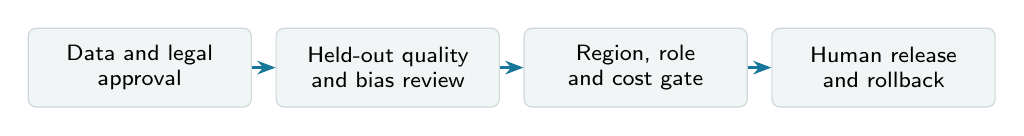
\begin{tikzpicture}[>=Stealth,every node/.style={font=\sffamily\fontsize{7.7}{9}\selectfont},n/.style={draw=thinrule,rounded corners=1mm,fill=papergray,align=center,text width=26mm,minimum height=10mm}]
\node[n](a){Data and legal\\approval};\node[n,right=3mm of a](b){Held-out quality\\and bias review};\node[n,right=3mm of b](c){Region, role\\and cost gate};\node[n,right=3mm of c](d){Human release\\and rollback};
\draw[->,thick,steelblue](a)--(b);\draw[->,thick,steelblue](b)--(c);\draw[->,thick,steelblue](c)--(d);
\end{tikzpicture}\\{\fontsize{8}{9}\selectfont\color{inkgray}Figure 14.4. A model is released only after independent quality and control gates.}\end{center}
\textbf{Wrong-task risk.} A text generation model cannot establish the underlying physical cause of a turbine trip without calibrated evidence; an apparent causal explanation may only paraphrase a technician's initial suspicion. Keep diagnostic statements, recommendations and factual events separate in the application schema. Distinguish ``operational support'' from autonomous control of physical equipment.

\textbf{Misleading benchmark risk.} A clean 35-row synthetic experiment says nothing about cold starts, high-wind curtailment, seasonality shifts, meter downtime or the thousands of correlated hourly observations in a real system. Confidence claims must match observed scope. Any live pilot should add backtesting over multiple months or seasons, a change-detection plan and escalation when data is incomplete.

\textbf{Review protocol.} For every failure case, record the expected behaviour, actual behaviour, severity, responsible reviewer and decision. If the model repeatedly cites unsupported facts, disable narrative explanations while keeping verified numerical views online. If live forecasting beats the baseline only on one unusually easy week, decline promotion until independent slices confirm the gain.
\begin{insight}\textbf{Responsible AI is also a reliability discipline.} Every AI component needs the same operational obligations as the rest of the data platform: an owner, a minimum test suite, monitoring, versioned outputs, security boundaries, a fallback and an explicit withdrawal criterion.\end{insight}
\repo{P170: Cortex agent evaluations}{https://github.com/Snowflake-Labs/sfguide-getting-started-with-cortex-agent-evaluations}

\newpage

% PAGE 261
\section*{14.8\quad Token usage, compute charges, and AI cost controls}
\topic{14.8.1}{Tokens are not queries, and neither is a fixed bill}
AI inference services frequently charge according to model-dependent input/output token consumption, page counts or other usage units. The same prompt repeated against many data rows can multiply cost, and a model producing a long response can be materially dearer than one returning a short validated label. A retrieval system has additional indexing and ongoing serving considerations; model training and Snowpark transformations may consume warehouse or serverless compute.

Treat cost as several meters, not a single undifferentiated credit figure. For AI SQL, log request count, model, input units, output units, timestamp, status and charge source. For search services, include index refresh, embeddings, serving footprint and source-query compute. For ML functions, include training and inference compute with edition-specific behaviour. Avoid adding a guessed ``EUR per prompt'' without the applicable consumption table and contractual credit rate.
\topic{14.8.2}{A cost formula that remains valid when rates change}
A useful illustrative token model is
\[
C_{\mathrm{tokens}} = \sum_{m}\left(\frac{I_m}{10^{6}}r^{\mathrm{in}}_m + \frac{O_m}{10^{6}}r^{\mathrm{out}}_m\right),
\]
where $I_m$ and $O_m$ are observed input/output token totals for model $m$, and $r_m$ are the applicable \emph{date- and region-specific} credit rates per million tokens. If the meter is pages, compute pages at the published page rate instead; do not force everything into tokens. Credits and the organisation's currency conversion must be recorded separately.
\begin{whitebox}\textbf{Hypothetical sizing example (not a quote).}\par
An approved dry run considers 1{,}000 calls, an estimated 400 input tokens and 60 output tokens per call: 0.40 million input and 0.06 million output tokens. The illustrative formula is $0.40r^{\mathrm{in}}+0.06r^{\mathrm{out}}$ credits \emph{before} other compute. No monetary or actual credit total is claimed until rates and measurements are obtained.
\end{whitebox}
\repo{P173: Cortex cost governance reference}{https://github.com/sfc-gh-tdahlberg/cortex-cost-governance}

\newpage

% PAGE 262
\topic{14.8.3}{Enforce exposure limits before the first batch}
Snowflake publishes account-usage views such as \texttt{CORTEX\_AI\_}\allowbreak\texttt{FUNCTIONS\_USAGE\_}\allowbreak\texttt{HISTORY} for AI function monitoring. Data availability and latency may vary; consult the current schema before writing a production report. Budget alerts and usage dashboards are useful, but they are not by themselves guaranteed hard caps on every AI request. Resource monitors largely address warehouse usage rather than every serverless AI meter. The practical control is a combination of scoped privileges, approved workload size, query tagging, request throttling, alerting and a tested stop path.
\begin{lstlisting}[language=SQL]
-- Read-only example: inspect available usage metadata.
SELECT *
FROM SNOWFLAKE.ACCOUNT_USAGE.CORTEX_AI_FUNCTIONS_USAGE_HISTORY
LIMIT 10;
-- Requires rights; schema/latency can change over time.
\end{lstlisting}
\textbf{Guardrail design.} (1) Begin with 10 synthetic test cases. (2) Estimate worst-case prompt growth and generated length. (3) Approve a finite number of rows. (4) Use an explicit timeout and retry limit. (5) Monitor measured consumption. (6) Define who can revoke the AI role or stop scheduled jobs. (7) Require reapproval for new models, regions or larger batches.\par
\textbf{Failure example.} A scheduled report generates a new summary for every record at every refresh, even when the underlying note has not changed. The query is functionally correct, but compute and token usage scale with reprocessing, not new information. Cache only permitted, versioned results when freshness requirements allow, and keep an auditable invalidation policy when source content changes.
\begin{insight}\textbf{Cost and security link.} A permissive AI execution role is a spending risk. If any analyst can run unrestricted model invocations against a large table, dashboards cannot guarantee that the credit bill remains within an informal target. Restrict the capability by role and explicitly review batch size before enabling recurring schedules.\end{insight}
\textbf{Check.} List which meters your proposed workload actually exercises, which ones a given monitor can affect and what human or automated intervention ends a runaway experiment.
\repo{P174: AI observability guided example}{https://github.com/Snowflake-Labs/sfguide-getting-started-with-ai-observability}

\newpage

% PAGE 263
\section*{14.L\quad Guided lab, chapter review, and exercises}
\topic{14.L.1}{Goal, prerequisites, permissions and safeguards}
\textbf{Goal.} Compare an interpretable one-day energy forecast with a second baseline and identify an injected anomaly; construct an evaluation specification for an optional, paid AI explanation without actually calling any model. The offline path is entirely synthetic, has no credential requirement, and incurs no Snowflake bill. Optional Snowflake exercises require a restricted sandbox role, administrator approval of region and model, time limits and measured usage.

\textbf{Inputs.} The companion package contains \texttt{ml\_baseline.py}, a generated daily CSV, a model card, labelled AI cases, optional SQL, unit tests and a README. The generator builds 35 UTC days with a weekly pattern, deliberately small variation and a +6 MWh spike on day index 34. This extended series is a \emph{new synthetic test fixture}, separate from the six 66.000 MWh observations in Chapters~8--13.
\topic{14.L.2}{Reproduce the baseline and examine the outputs}
\begin{lstlisting}[language=bash]
# At the lab directory; Python 3.10+; no packages needed:
python ml_baseline.py
python -m unittest discover -s tests -v
\end{lstlisting}
\textbf{Procedure.} (1) Inspect the CSV and confirm the daily UTC key and declared synthetic provenance. (2) Verify that training, validation and test days are strictly chronological. (3) Calculate last-value and lag-7 seasonal forecasts. (4) Derive the residual alert threshold using validation days alone. (5) Score the final seven days exactly once. (6) Inspect the flagged spike and explain why a single synthetic outlier is not an operational accuracy claim. (7) Complete the model card with deployment objections.
\begin{whitebox}\textbf{Observed result in the supplied offline test environment}\par
Train / validate / test: 21 / 7 / 7 daily points. Seasonal test MAE: \textbf{1.0643 MWh}; last-value test MAE: \textbf{3.2500 MWh}. Residual threshold: \textbf{0.8500 MWh}. The test spike at day index 34 is flagged; an otherwise identical series with no injected spike does not flag that final day. All 16 Python \texttt{unittest} cases pass. These figures are deterministic synthetic results, \emph{not} Cortex or Finnish grid measurements.
\end{whitebox}

\newpage

% PAGE 264
\topic{14.L.3}{Assertions, diagnosis, rollback and cleanup}
Core acceptance checks: 35 unique contiguous UTC dates; only synthetic input; nonnegative finite values; past-only lag features; no test-derived threshold; expected held-out MAE; a flagged injected spike; and rejection of duplicate dates, negative values and unexpected provenance. The accompanying tests verify these invariants. The default SQL file is read-only or commented where billable examples would otherwise run.

\textbf{If a test fails:} a duplicate date means the business grain is broken; an unexpected model score may indicate future leakage or fixture drift; a spurious anomaly may reflect an improperly calibrated threshold; an access error in a proposed Cortex call requires a privileges/region check, not an administrator-privilege shortcut. Roll back by returning to the validated fixture and versioned baseline, disabling optional calls, and retaining evidence. Cleanup needs only deletion of disposable local output files; destructive Snowflake cleanup statements are deliberately omitted.
\topic{14.L.4}{Review questions, exercises and design rubric}
\textbf{Concept checks.} (1) Why is SQL a better fit for an exact MWh total than text generation? (2) How can a forecast feature leak future information? (3) What distinguishes retrieved evidence from a grounded claim? (4) Why is storing data in the EU insufficient to prove inference stays there? (5) Which AI expenses may remain outside ordinary warehouse resource monitors?

\textbf{Foundation exercise.} Reproduce both holdout MAEs, show the individual test residuals and explain the intentional anomaly. \emph{Acceptance:} matching values, correct units and a clear synthetic-data disclaimer.

\textbf{Practitioner exercise.} Create an additional missing-day case and adapt the series validator to reject it without interpreting it as zero production. Add two labelled AI evaluation cases: one note with insufficient evidence and one note attempting a prompt override. \emph{Acceptance:} explicit rejection conditions and unchanged baseline splits.

\textbf{Architectural decision.} A team asks for automated explanations of future energy shortage events. Recommend deterministic rules, forecasting, RAG and/or Cortex functions. Document access, residency, human review, true evaluation criteria and a financial stop policy. \emph{Acceptance:} an inspectable alternative comparison, a versioned test plan and no claims of untested model performance.
\begin{whitebox}\textbf{Rubric (20 points).}\par
Task-to-method reasoning (4); chronological validation and reproducibility (5); grounded evaluation and responsible deployment (5); region/role/cost controls (4); explicit limitations and provenance (2). Pass at 16 or above with no invented measured credit charge or fabricated evidence.
\end{whitebox}
\textbf{Chapter synthesis.} AI can enrich a governed data platform, but cannot excuse a weak baseline, missing provenance or uncontrolled expense. In Chapter~15 the same discipline will turn the evolving Finland Energy Analytics example into a capstone whose outputs, operational decisions and limitations are auditable.
{\fontsize{7.6}{9}\selectfont\textbf{Technical references (checked 22 October 2026).} \href{https://docs.snowflake.com/en/sql-reference/functions/ai_complete}{[1] AI COMPLETE}; \href{https://docs.snowflake.com/en/user-guide/snowflake-cortex/cross-region-inference}{[2] Cross-region inference}; \href{https://docs.snowflake.com/en/user-guide/snowflake-cortex/cortex-search/cortex-search-overview}{[3] Cortex Search}; \href{https://docs.snowflake.com/en/sql-reference/classes/forecast/commands/create-forecast}{[4] Forecast ML}; \href{https://docs.snowflake.com/en/user-guide/snowflake-cortex/ai-func-cost-management}{[5] AI cost management}. \textit{Referenced GitHub projects are not executed or cleared for republication.}}

\end{document}
